\section{Introduction}
Penguin ASI is a robotics firm engaged in the development of automation strategies for the mining industry and the development of telerobotic systems to work in extreme and hazardous environments. As the use of automated technology becomes more prevalent in the mining industry there comes a need to develop a telecommunications network. In order to prevent the need to retrofit an existing mine with a communications network, Penguin had developed an optical communications range extender and mounted it on a teleoperated, mobile platform to be able to relay the signals. The first iteration of this platform had some issues with its design that Penguin had wished to resolve in a second iteration prototype. In order to produce a functional prototype all issues with the previous version must have been addressed, and the robot must have been able to achieve certain functional requirements laid out by the client, Penguin ASI.  
\section{Problem Statement}
The initial communications robot produced by Penguin ASI had displayed many issues affecting its performance and needed to be addressed. Its operating environment was intended to include traversal through wet and rough terrain, which required all drive components to be sealed against water and dirt. To seal the original drive boxes gasket maker was used, but was inadequate and allowed water to enter the drive box as seen in Figure \ref{} 
 
\begin{figure}[H]
\centering
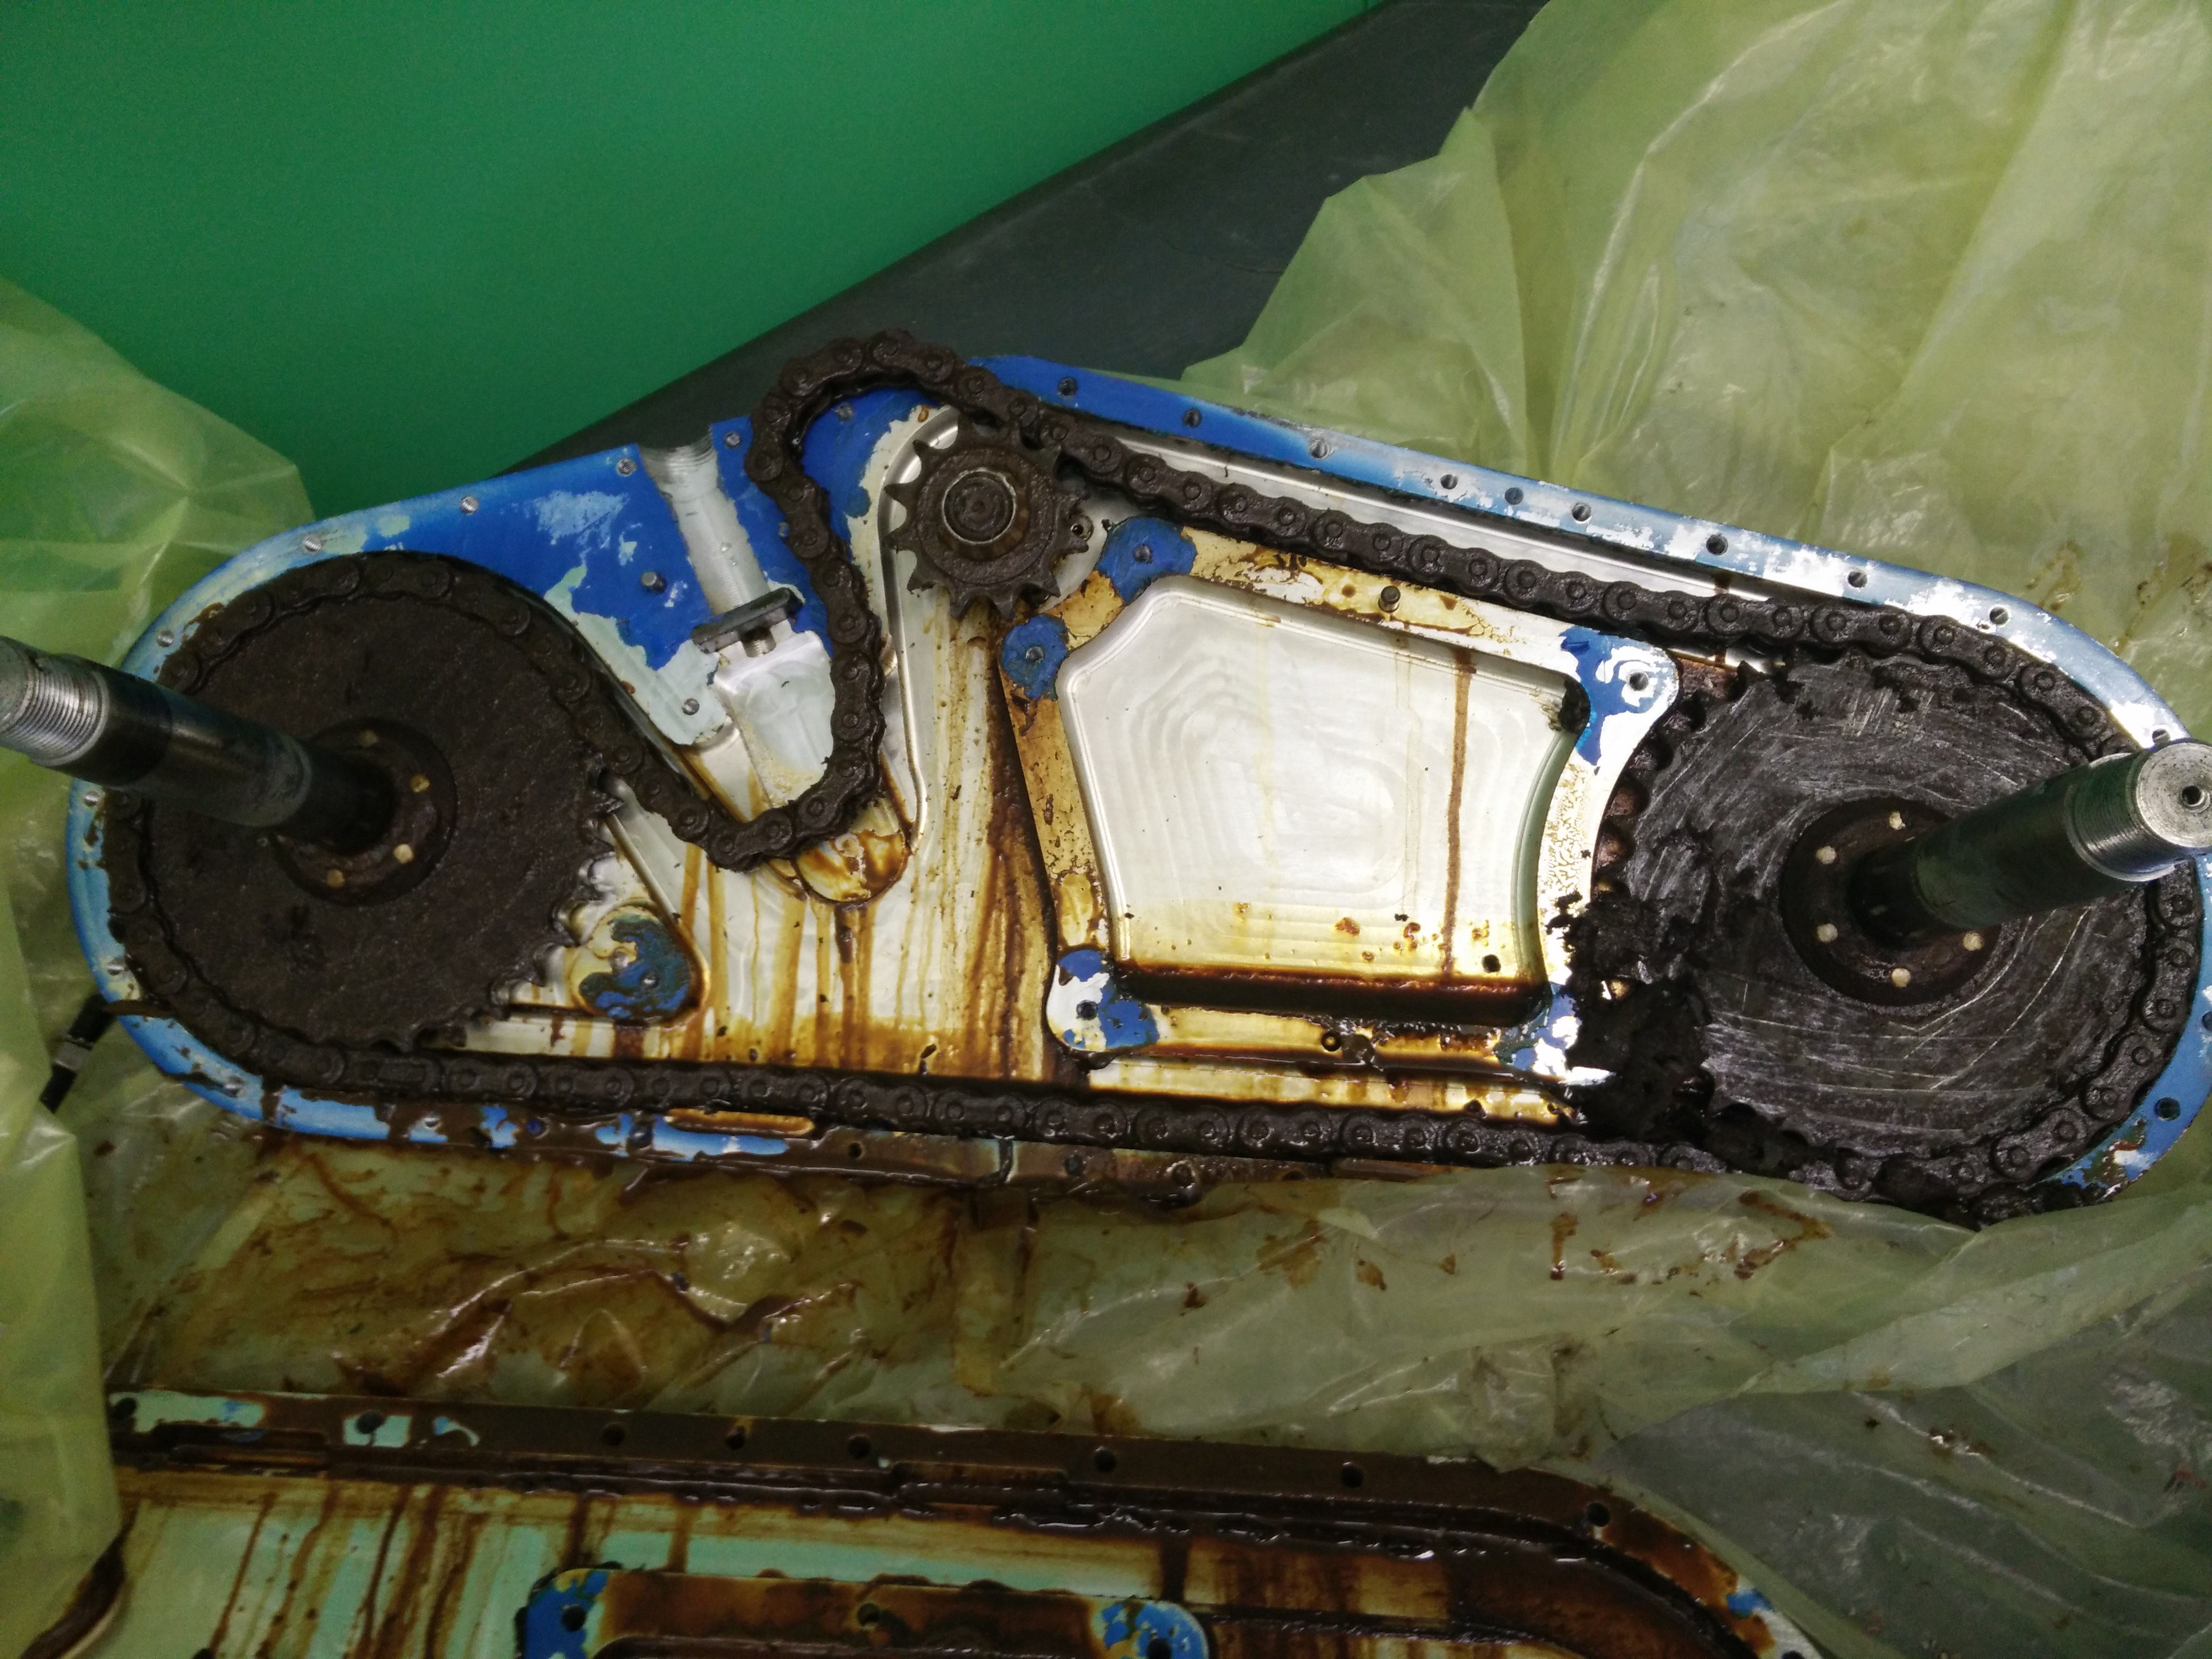
\includegraphics[width=0.5\linewidth]{./images/inside_drive_box_orig}
\caption{}
\label{fig:inside_drive_box_orig}
\end{figure}
 